\chapter[Problemas de teste]{Problemas de teste}

A fim de avaliar os métodos multiobjetivos, normalmente se utiliza problemas de teste. São vários os problemas em que se pode aplicar os algoritmos multiobjetivos, os quais podem ser divididos em duas categorias: contínuos ou discretos. Os problemas contínuos são funções contínuas e não necessariamente representam um problema real. Alguns exemplos de problemas contínuos (SCH, FON, POL, KUR e ZDT) podem ser encontrados no artigo original do NSGA-II \cite{Deb2002}. Os problemas discretos, por outro lado, possuem um enunciado bem definido e nem todas as soluções possíveis são válidas, ou seja, existem lacunas no contradomínio das funções. Exemplos de problemas discretos comummente usados na literatura multiobjetivo são: cacheiro viajante \cite{MTSP}, roteamento de veículos com janelas de tempo \cite{VehicleRouting}, problema da mochila \cite{MKP}, sequenciamento de proteínas \cite{Brasil2013} e problemas de roteamento em redes \cite{Lafeta2017}. O comportamento e a adequação ao uso de um determinado algoritmo multiobjetivo são influenciados pelo tipo do problema. Neste trabalho, dois problemas discretos foram investigados: o problema da mochila multiobjetivo (PMM) e o problema do roteamento multicast (PRM), os quais são descritos a seguir.

\section{Problema da mochila multiobjetivo}

O \ac{PM} é um problema muito comum na computação e possui um caráter teórico. Entretanto, existem problemas reais equivalentes que podem ser resolvidos com as mesmas técnicas, como o escalonamento de tarefas em um sistema operacional.

O problema consiste em arranjar um conjunto de itens em uma mochila de forma a não exceder sua capacidade e, ao mesmo tempo, maximizar o valor (lucro) dos objetos carregados. Matematicamente, dada uma mochila de capacidade $C$ e um conjunto de itens $O$, onde cada $o_i \in O$ possui um peso $peso(o_i)$ e um lucro $lucro(o_i)$, encontrar o conjunto $S \subset O$, tal que $\sum_{o \in S} peso(o) \leq C$ e $\sum_{o \in S} lucro(o)$ seja o maior possível. A \autoref{fig_knapsack} mostra uma instância do problema da mochila mono-objetivo e três soluções possíveis.

\begin{figure}[!htbp]
	\centering
	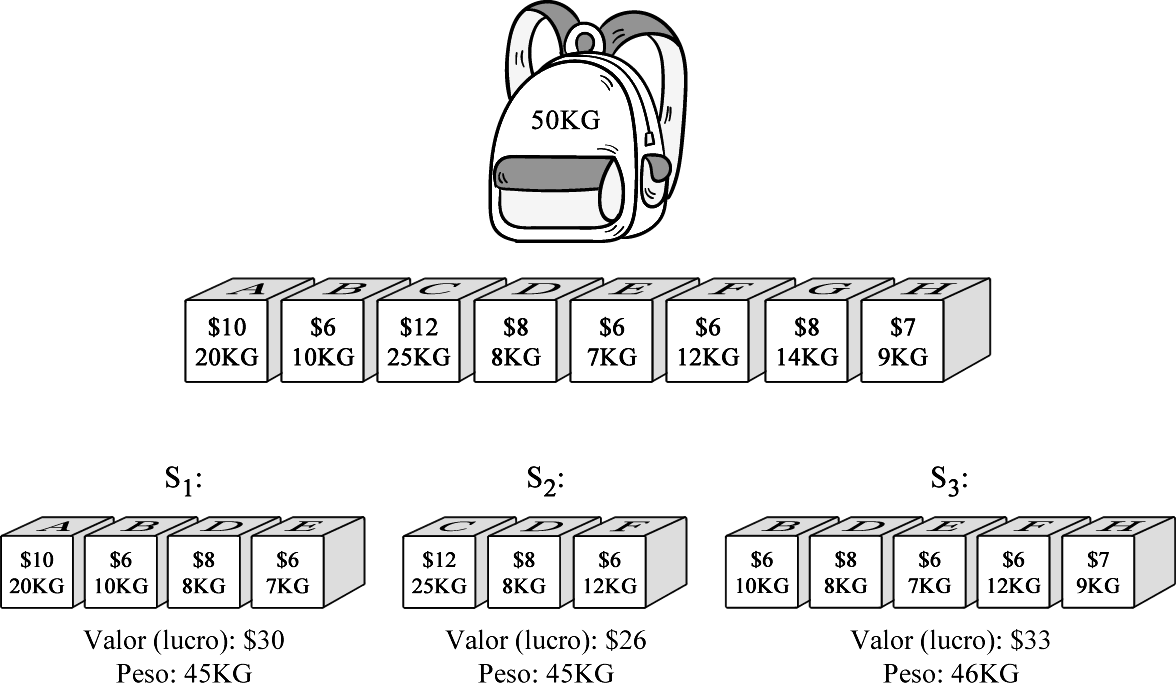
\includegraphics[width=1\textwidth]{cap_problemas/figs/mochila.png}
	\caption{\label{fig_knapsack}Exemplo para o problema da mochila mono-objetivo.}
\end{figure}

Na \autoref{fig_knapsack}, a capacidade máxima da mochila é 50Kg e existem oito itens disponíveis para se escolher. Três soluções possíveis são mostradas ($S_1$, $S_2$ e $S_3$), dentre elas, a melhor é $S_3$, pois possui o maior valor de lucro e ao mesmo tempo é válida, ou seja, repeita a restrição de capacidade (peso menor que 50Kg). No exemplo, todas as soluções estão saturadas, em outras palavras, a adição de qualquer outro item as tornam inválidas.

Existem diversas estratégias para resolver o \ac{PM}. Dentre elas, as mais usadas são os algoritmos gulosos \cite{KnapsackGreedy}, a programação dinâmica \cite{KnapsackDynamic} e os algoritmos genéticos \cite{KnapsackGA}. Os algoritmos gulosos e a programação dinâmica são os mais rápidos e eficientes para resolver o PM mono-objetivo. Em contra-partida, a complexidade adicionada ao considerar mais de um objetivo inviabiliza a utilização desse tipo de algoritmo, tornando os algoritmos genéticos e demais métodos bio-inspirados as melhores opções.

O problema da mochila multiobjetivo (PMM) é similar ao original. Sua única diferença está no fato de que cada item, ao invés de possuir um único valor (lucro), é composto de múltiplos valores. No PMM, a função $lucro(o_i)$ retorna um vetor ao invés de um único valor escalar. Cada componente (elemento) do vetor representa o valor do item $o_i$ considerando um dos objetivos. Por exemplo, considerando um PMM de 3 objetivos, cada $o_i \in O$ possui um vetor formado por três valores de lucros (um para cada objetivo). O objetivo do problema passa a ser maximizar todos os lucros ao invés de um único valor.

O PMM já foi utilizado várias vezes para avaliar algoritmos multiobjetivos, podendo-se destacar os trabalhos de \cite{Zitzler1999}, \cite{Zitzler2002} e \cite{Zhang2007}. As instâncias do PMM utilizadas no decorrer deste trabalho foram geradas de forma aleatória e compreendem problemas da mochila com 30, 40, 50, 100 e 200 itens. Para gerar as instâncias, sorteou-se valores no intervalo (0, 1000) para os lucros e para os pesos. A capacidade da mochila foi sempre definida como 60\% da soma dos pesos.  

\section{Problema do roteamento multicast}
\label{section_problemas_prm}

O problema do roteamento multicast (PRM) aparece na engenharia de tráfego em redes de computadores e consiste em escolher a forma ``mais eficiente'' de transmitir uma mensagem multicast \cite{Lafeta2016}. Uma transmissão de rede pode ser do tipo unicast, multicast ou broadcast. Em transmissões unicast, conecta-se um ponto da rede a outro ponto qualquer (transmissão ponto-a-ponto). Para fazer isso de forma eficiente, basta usar algum algoritmo capaz de encontrar o melhor caminho entre os dois pontos (e.g. \cite{Dijkstra1959}). As comunicações broadcast caracterizam-se pelo fato de um nó da rede (servidor) enviar o conteúdo a todos os demais. Para obter as melhores rotas para trafegar os dados, basta utilizar algum algoritmo capaz de determinar a árvore geradora de custo mínimo (e.g. \cite{Prim1957}). Em uma comunicação multicast, o objetivo é transmitir o conteúdo de um nó da rede, chamado nó de origem ou transmissor, para alguns outros nós, denominados receptores. Essa tarefa apresenta maior complexidade, pois é necessário obter uma árvore de Steiner de custo mínimo, o que é mais difícil que calcular uma única rota ou construir a árvore geradora de custo mínimo \cite{Bueno2010}.

O PRM é um problema prático muito importante. Seu estudo visa o desenvolvimento de algoritmos eficientes e eficazes, proporcionando avanços na geração de rotas em redes de computadores. O objetivo desses algoritmos é encontrar soluções (rotas multicast) que permitam uma comunicação mais rápida, menos custosa e mais confiável entre dispositivos, o que é essencial em uma era onde a maioria das pessoas consomem informação e entretenimento pela Internet.

Dado que deseja-se transmitir um conteúdo via uma rede de computadores, o problema consiste em encontrar a melhor rota possível entre a fonte de dados e os vários destinos. dado um grafo $G=(V,E)$ que representa a rede de comunicação, um nó raiz $s \in V$ (nó transmissor) e um conjunto de nós destinos $D \subset V$ (nós receptores), o PRM consiste em determinar a subárvore $T$ de $G$ enraizada em $r$ que inclui todos os vértices em $D$ e apresenta o menor custo possível. A \autoref{fig_prm_grafo} ilustra uma instância do problema de roteamento multicast. Nesse exemplo de rede de comunicação, o nó receptor é definido por um círculo duplo (vértice 0), os nós receptores são destacados em cinza escuro (vértices 1, 8, 12 e 13) e os nós intermediários estão em cinza claro. Os números em cada aresta determina o custo da comunicação entre os nós que ela conecta.

\begin{figure}[!htbp]
	\centering
	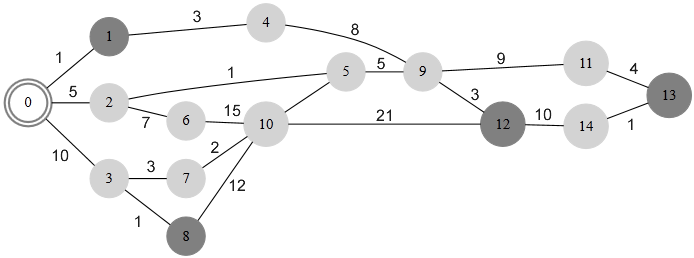
\includegraphics[width=1\textwidth]{cap_problemas/figs/prm_grafo}
	\caption{\label{fig_prm_grafo}Exemplo de uma rede de comunicação. Retirado de \cite{BuenoThesis}}
\end{figure}

Na \autoref{fig_prm_mono} são apresentados alguns exemplos de árvores multicast criadas a partir do grafo mostrado na figura \autoref{fig_prm_grafo}. O custo de cada árvore é dado pela soma dos custos de suas arestas. Dentre os exemplos, a árvore mais à direita possui o menor custo total: 65.

\begin{figure}[!htbp]
	\centering
	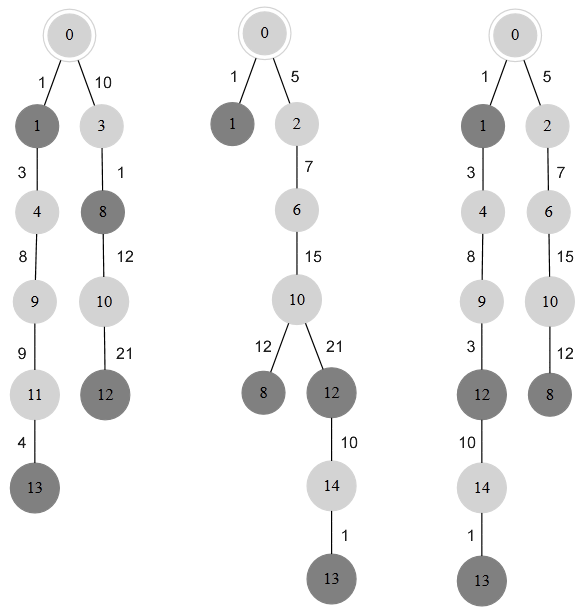
\includegraphics[width=0.8\textwidth]{cap_problemas/figs/prm_mono}
	\caption{\label{fig_prm_mono}Exemplos de árvores multicast relativos ao grafo da figura \autoref{fig_prm_grafo}. Retirado do trabalho de \cite{LafetaThesis}}
\end{figure}

O PRM original é proposto com apenas um objetivo a se otimizar, entretanto, essa não é uma visão realista do problema. A qualidade de um enlace de rede não pode ser medida através de uma única métrica, ou seja, um custo genérico não é capaz de determinar se um link é bom ou ruim. Características como distância, atraso (\textit{delay}), capacidade de tráfego e uso do tráfego são boas métricas da qualidade de serviço (QoS) em uma comunicação \cite{LafetaThesis}. 

Nesse contexto, este trabalho investiga uma versão multiobjetivo do problema de roteamento multicast. Nesta versão do problema, as árvores apresentadas como solução devem representar o melhor compromisso entre as métricas utilizadas.

\begin{figure}
	\centering
	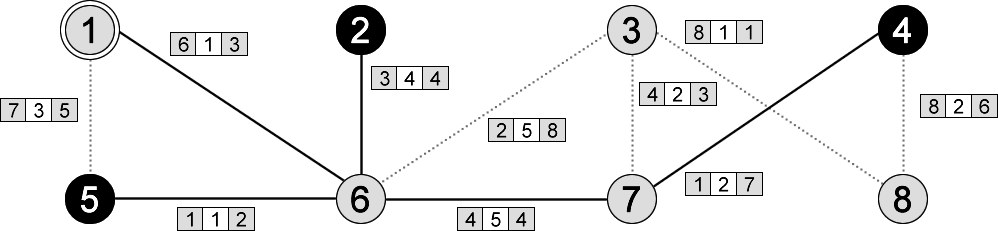
\includegraphics[width=1\textwidth]{cap_problemas/figs/prm_multi}
	\caption{\label{fig_prm_multi}Exemplo de árvore multicast no PRM multiobjetivo. Retirado de \cite{Bueno2010}}
\end{figure}

Na \autoref{fig_prm_multi} é apresentado um exemplo de rede com as métricas ``custo'' (primeiro valor) e ``delay'' (segundo valor) nas arestas. As arestas em negrito representam uma árvore multicast ótima (não-dominada) para o seguinte conjunto de objetivos \cite{Lafeta2016}:

\begin{enumerate} 
	\item Minimizar o custo total, que corresponde à soma dos valores de custo de todas as arestas da árvore.
	\item Maximizar o atraso (\textit{delay}) fim-a-fim atendidos, ou seja, o número de ramos da árvore em que a soma dos \textit{delays} nas arestas não ultrapassa um valor $d_{max}$ pré-definido, neste caso 25. Em outras palavras, quantidade de conexões cliente-servidor que mantém o limite aceitável de atraso.
\end{enumerate}

Neste trabalho considera-se até quatro valores de peso para um enlace da rede: custo, \textit{delay}, capacidade de tráfego e tráfego corrente, representados respectivamente pelas funções: $c()$, $d()$, $z()$ e $t()$. Por meio dessas medidas são formulados os seguintes objetivos:

\begin{enumerate} 
	\item \textbf{Custo total:} soma dos valores de custo de todas as arestas da árvore.
	\item \textbf{Delay fim-a-fim médio:} média da soma dos \textit{delays} em cada ramo da árvore. Em outras palavras, média do atraso em cada uma das comunicações cliente-servidor.
	\item \textbf{Delay fim-a-fim máximo:} maior valor para a soma de \textit{delays} dentre todos os ramos da árvore, ou seja, o maior atraso dentre todas as comunicações cliente-servidor.
	\item \textit{Hops count}: número de vértices na árvore.
	\item \textbf{Utilização máxima de enlaces:} considerando todas as arestas na árvore, qual delas atinge a maior utilização de banda? Matematicamente, considerando $E$ o conjunto de arestas da árvore e $\phi$ o tamanho da mensagem, essa métrica é dada por: \[\max_{e \in E} \frac{t(e) + \phi}{z(e)}\]
	\item \textbf{Utilização média dos enlaces:} média da utilização de banda entre todas as arestas da árvore. Seu cálculo é similar ao da métrica anterior (utilização máxima de enlaces) e é dado por: \[\frac{\sum_{e \in E} \frac{t(e) + \phi}{z(e)}}{|E|}\]
\end{enumerate}

A fim de possibilitar diversos cenários de teste para o PRM, os objetivos acima podem ser combinados de diversas maneiras, criando vários ambientes multi-objetivos. Neste trabalho foram utilizadas 5 formulações (combinações) desses objetivos:

\begin{enumerate}
	\item $P_2$: formado pelos objetivos 1 e 3.
	\item $P_3$: formado pelos objetivos 1, 3 e 4.
	\item $P_4$: formado pelos objetivos 1, 3, 4 e 5.
	\item $P_5$: formado pelos objetivos 1, 3, 4, 5 e 6.
	\item $P_6$: formado pelos objetivos 1, 2, 3, 4, 5 e 6.
\end{enumerate}

O PRM foi trabalhado sobre 5 redes diferentes variando a complexidade em termos de quantidade de nós destinos, vértices e arestas. Essas redes foram retiradas do trabalho de \cite{Lafeta2016} e suas caraterísticas são apresentadas na tabela \ref{tab_prm_redes}.

\begin{table}[!htbp]
	\centering
	\caption{Definições das redes utilizadas no PRM}
	\label{tab_prm_redes}
	\begin{tabular}{r|rrr}
		Nome        & Destinos & Vértices & Arestas \\ \hline
		Rede 1 (R1) & 10       & 33       & 106     \\
		Rede 2 (R2) & 18       & 75       & 188     \\
		Rede 3 (R3) & 37       & 75       & 188     \\
		Rede 4 (R5) & 12       & 75       & 300     \\
		Rede 5 (R5) & 16       & 100      & 250     \\ \hline
	\end{tabular}
\end{table}
